\section{State of the Art}

En la actualidad se está implementando el primer observatorio virtual chileno
para los datos del Atacama Large Milimeter/submilimeter Array (ALMA), quien
busca poder entregar sus datos científicos a la comunidad astronómica Chilena y
del mundo. Este proyecto se realiza en colaboración a cinco universidades
chilenas: Universidad Técnica Federico Santa María, Universidad de Chile,
Pontificie Universidad Católica, Universidad de Concepción y la Universidad de
Santiago de Chile. También participa la Red Universitaria Nacional (REUNA) y el
Centro de Modelamiento Matemático (CMM).

\subsection{Astronomical Data}
%avalancha de datos
Los telescopios e instrumentos en la astronomía, están afectos a los avances
tecnológicos. Este aspecto a nivel de información es muy provechoso, ya que
logran captar datos que antes no existían. Sin embargo computacionalmente la
preocupación está centrada en el crecimiento de los volúmenes de datos
generados, que ya pasó de los gigabytes a los terabytes en la decada pasada, y
que pasará de los terabytes a petabytes en la actual década. Por ejemplo:
\begin{itemize}
	\item Galaxy Evolution Explorer (GALEX): es un telescopio orbitante en
el espacio, que observa galaxias en luz ultra violeta. Se espera que genere 30
TeraBytes de Datos.
	\item Sloan Digital Sky Survey (SDSS): es un proyecto de inspección de
imágenes en el espectro visible y de corrimiento al rojo. Se espera que genere
40 TeraBytes de Datos.
	\item Atacama Large Milimeter/submilimeter Array (ALMA): es un
interferómetro que trabaja con 66 radio telescopios de platos de distintos
tamaños, obteniendo datos de radio, polarización, etc. Se espera que genere 1
TeraBytes de Datos por día de observación.
	\item Panoramic Survey Telescope \& Rapid Response System (Pan-STARRS):
es un sistema que permitirá obtener imágenes a gran campo de manera contínua.
Su objetivo es caracterizar objetos que se aproximen a la tierra, como
asteroides, cometas, etc. Se espera que genera 40 PetaBytes de datos.
\end{itemize}

Se podrían seguir listando observatorios, pero en conclusión, existe una
avalancha creciente de datos astronómicos, los cuales están cambiando la forma
en que se hace astronomía. Del punto de vista computacional, es necesario
implementar servicios estandares que permitan acceder, procesar, modelar los
datos producidos de cada observatorio (que generen datos públicos) de forma
estándar, naciendo así la idea de Observatorio Virtual. Los estándares y
protocolos de como operar están a cargo de la International Virtual Observatory
Allience. 

\subsection{Virtual Observatory}
El observatorio virtual no es un paquete de software (escritorio o web) que
permite acceder a los usuarios a los datos como si fuese un repositorio, que es
lo que generalmente se esperaría al escuchar la palabra. Técnicamente un VO
puede ser descrito como una arquitectura integral, que formaliza en cada
nivel de la aplicación los estándares y protocolos necesarios, de tal manera
que los VO del mundo sean interoperables entre si. Por lo tanto, cuando un
observatorio tiene datos para publicar no será necesario inventar una nueva
arquitectura, sino que se puede aprovechar la ya existente.

Por este motivo nace el año 2002 la International Virtual Observatory Alliance,
cuya misión es facilitar la coordinación y colaboración necesaria para
facilitar el acceso global e integrado a los datos recodigos por los
observatorios astronómicos internacionales. En esta organización están
comprometidos 19 VO actualmente, los cuales trabajan mediante working groups en
la creación y versionamiento de estándares y protocolos que comprende su
arquitectura.

\subsection{VO Architecture}

IVOA propone tres niveles de arquitectura, los cuales se pueden describir
dentro del Nivel 2, ya que el grado de especificación va aumentando.

\begin{figure*}[h!t]
    \centering
    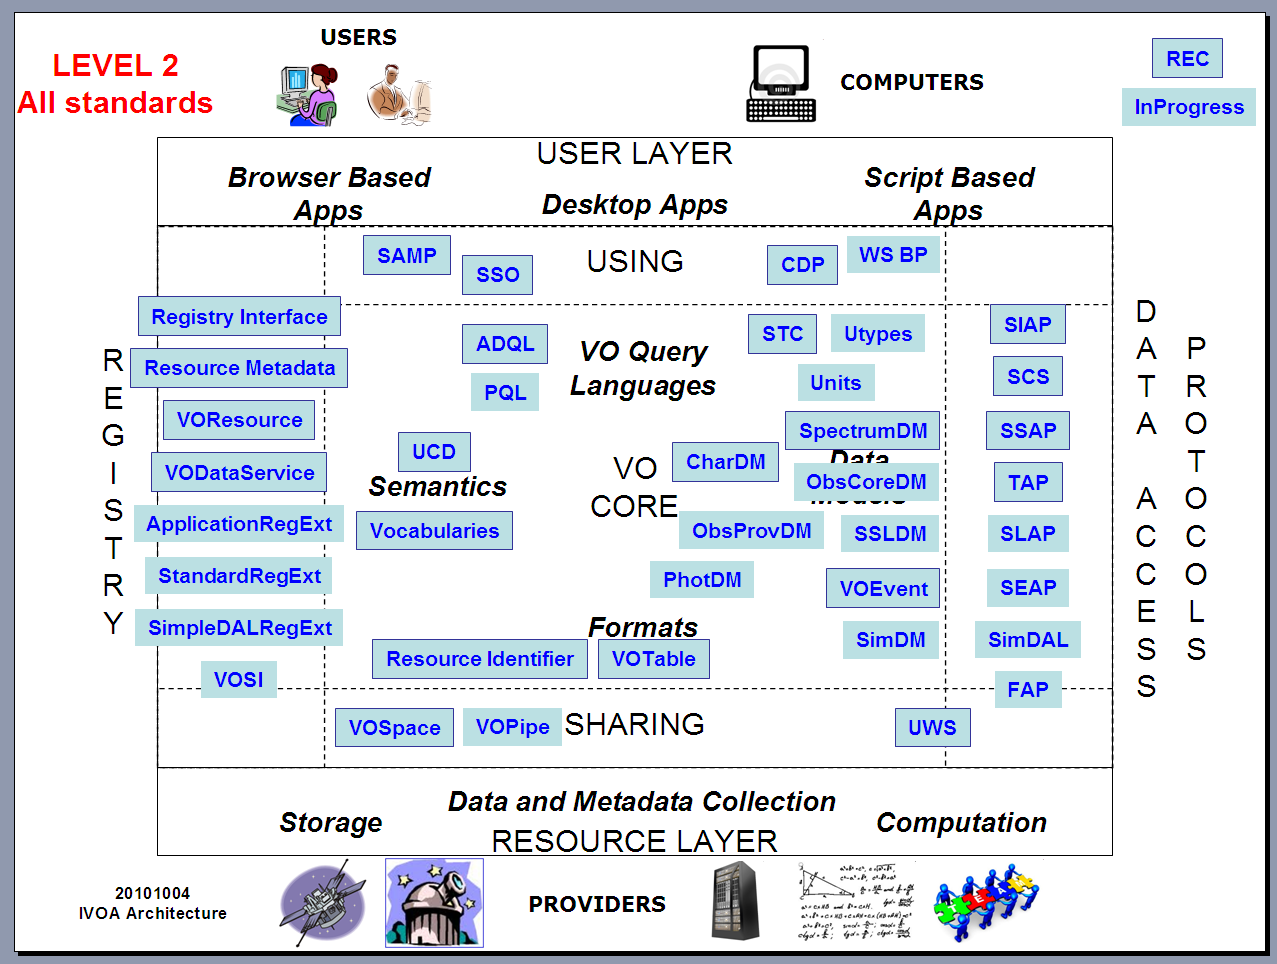
\includegraphics[width=0.7\textwidth]{img/arquitectura_2.png}
    \caption{Arquitectura Nivel 2}
    \label{fig:nivel2}
\end{figure*}

En esta definición, se identifican principalmente 3 capas:
\begin{itemize}
	\item Resource Layer: compuesto por colección de datos y metadatos.
	\item User Layer: consumidores de datos a través de navegador,
aplicación de escitorio, etc.
	\item Middle Layer: esta capa es necesaria para conectar los dos
anteriores de forma transparente tanto para los usuarios como para los
publisher. En el gráfico también se pueden ver recuadros en azul, en diferentes
secciones, los que son los estándares que rige IVOA. Para este documento el
foco será la sección de \emph{Data Access Protocol} (sección al lado derecho de
la imagen).
\end{itemize}

%Capa de acceso de datos

%Estándares de acceso de datos
